\section{Results}

\subsection{ASR Model-Comparison Context}

Table~\ref{tab:asr_benchmark} reports the 258-row ASR benchmark context. The partial-encoder run has the strongest current aggregate CER and WER profile in this split. This is model-comparison context only; it does not by itself establish downstream safety.

\begin{table}[htbp]
\centering
\caption{Main ASR benchmark on the 258-row split. Source: \artifact{70_experiments/runs/janus_258_test_split_asr_cds_proxy/asr_cds_proxy_comparison.tsv}.}
\label{tab:asr_benchmark}
\begin{tabular}{lrrrr}
\toprule
Run & Rows & CER zh micro & WER zh jieba micro & High-risk missed \\
\midrule
Partial encoder & 258 & 15.04 & 21.53 & 4 \\
LoRA legacy best & 258 & 18.23 & 25.59 & 7 \\
Breeze ASR25 base & 258 & 22.72 & 30.39 & 30 \\
Breeze ASR26 & 258 & 24.27 & 32.29 & 22 \\
\bottomrule
\end{tabular}
\end{table}


\subsection{Predictor Comparison}

Table~\ref{tab:predictor} and Figure~\ref{fig:predictor_auc} compare WER, CER, SRES, and CEIS against human-reviewed decision-change labels. CEIS has the strongest point AUC in the scoped audit and reaches a zero-false-negative diagnostic operating point. This is reported as a decision-stability signal under the selected audit boundary, not as a deployment threshold or universal classifier claim.

\begin{table}[htbp]
\centering
\caption{Predictor performance against human-reviewed decision-change labels. Source: \artifact{human_audit_predictor_comparison.tsv}. Thresholds are diagnostic operating points on the scoped audit set.}
\label{tab:predictor}
\begin{tabular}{lrrrrr}
\toprule
Metric & AUC & Best threshold & F1 & Recall & FN \\
\midrule
WER & 0.6964 & 42.59 & 0.4615 & 0.5625 & 7 \\
CER & 0.7276 & 16.42 & 0.4516 & 0.8750 & 2 \\
SRES & 0.8995 & 270.00 & 0.6512 & 0.8750 & 2 \\
CEIS & 0.9117 & 5.00 & 0.6275 & 1.0000 & 0 \\
\bottomrule
\end{tabular}
\end{table}


\begin{figure}[htbp]
\centering
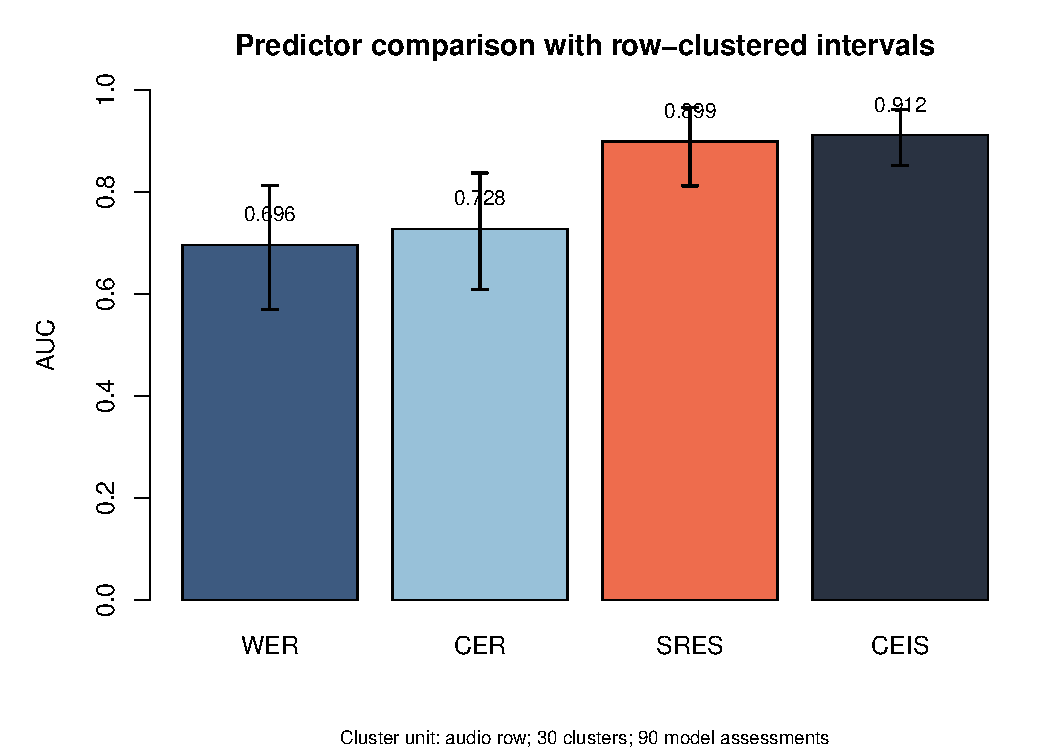
\includegraphics[width=.9\linewidth]{figures/fig3_predictor_auc.pdf}
\caption{Predictor comparison for WER, CER, SRES, and CEIS with row-clustered intervals. Source artifacts: \artifact{human_audit_predictor_comparison.tsv} and \artifact{human_audit_predictor_clustered_ci.tsv}.}
\label{fig:predictor_auc}
\end{figure}

\subsection{Aggregate Policy Replay}

Table~\ref{tab:policy} and Figure~\ref{fig:policy_replay} report aggregate policy replay. SRES-triggered recovery and CEIS-triggered conservative action eliminate high-risk missed and critical miss counts in aggregate replay at the same diagnostic budget. CEIS ensemble arbitration adds abstention behavior at a higher budget.

\begin{table}[htbp]
\centering
\caption{Aggregate policy replay under human-reviewed selected-300 labels. Source: \artifact{policy_comparison.tsv}.}
\label{tab:policy}
\small
\begin{tabularx}{\linewidth}{@{}Lrrrr@{}}
\toprule
Policy & Budget & Unsafe downrouting & High-risk missed & Critical miss \\
\midrule
No recovery & 0.0000 & 29 & 6 & 1 \\
Confidence only & 0.0000 & 29 & 6 & 1 \\
SRES recovery & 0.3889 & 24 & 0 & 0 \\
CEIS conservative action & 0.3889 & 24 & 0 & 0 \\
CEIS ensemble arbitration & 0.5222 & 24 & 0 & 0 \\
\bottomrule
\end{tabularx}
\end{table}


\begin{figure}[htbp]
\centering
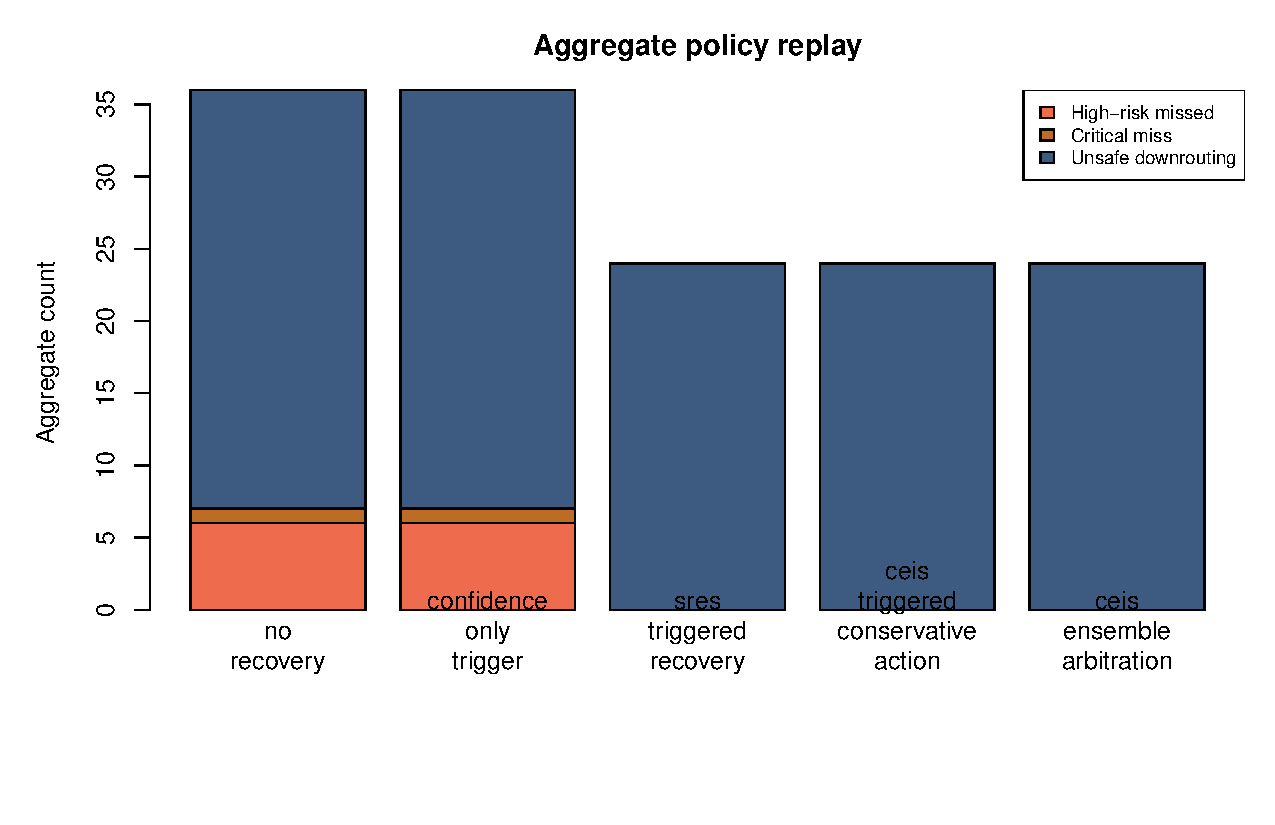
\includegraphics[width=.9\linewidth]{figures/fig4_policy_replay.pdf}
\caption{Aggregate policy replay under human-reviewed selected-300 labels. Source artifact: \artifact{70_experiments/runs/janus_300_high_stakes_recovery_human_reviewed_2026_05_26/policy_comparison.tsv}.}
\label{fig:policy_replay}
\end{figure}

\subsection{Fixed-Budget Frontier And Risk Atoms}

Figure~\ref{fig:frontier} shows the fixed-budget conservative replay frontier. Figure~\ref{fig:risk_atom} summarizes human-reviewed decision-change evidence by risk atom.

\begin{figure}[htbp]
\centering
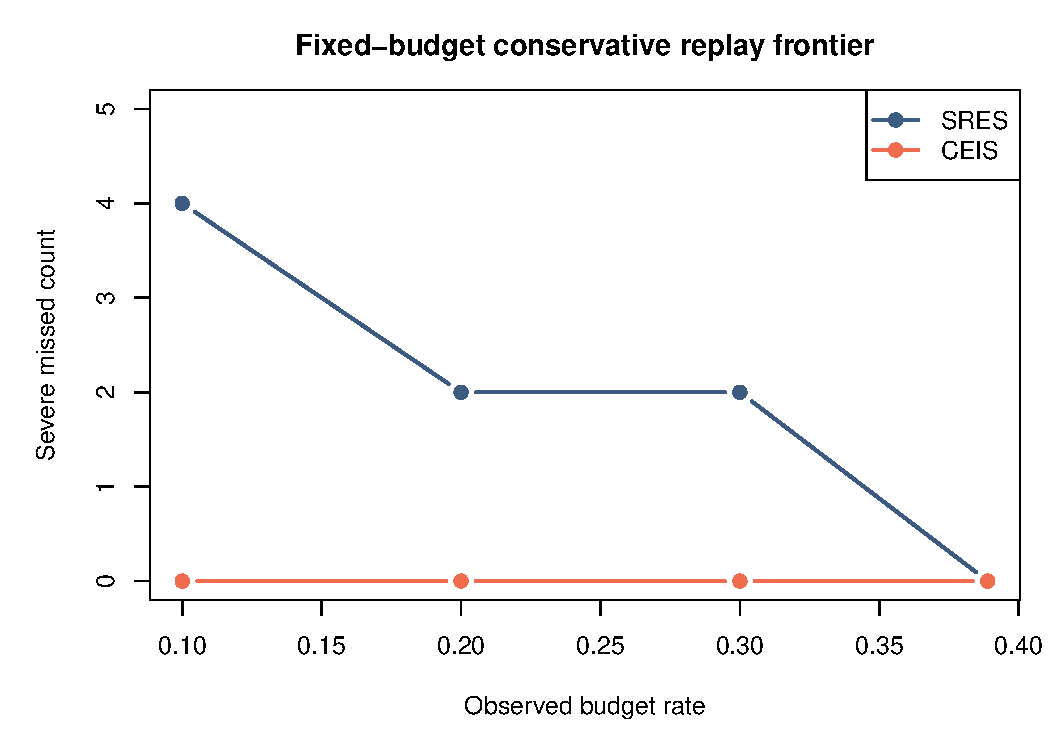
\includegraphics[width=.9\linewidth]{figures/fig5_fixed_budget_frontier.pdf}
\caption{Fixed-budget conservative replay frontier. Source artifact: \artifact{70_experiments/runs/janus_300_high_stakes_recovery_human_reviewed_2026_05_26/fixed_budget_recovery_frontier.tsv}.}
\label{fig:frontier}
\end{figure}

\begin{figure}[htbp]
\centering
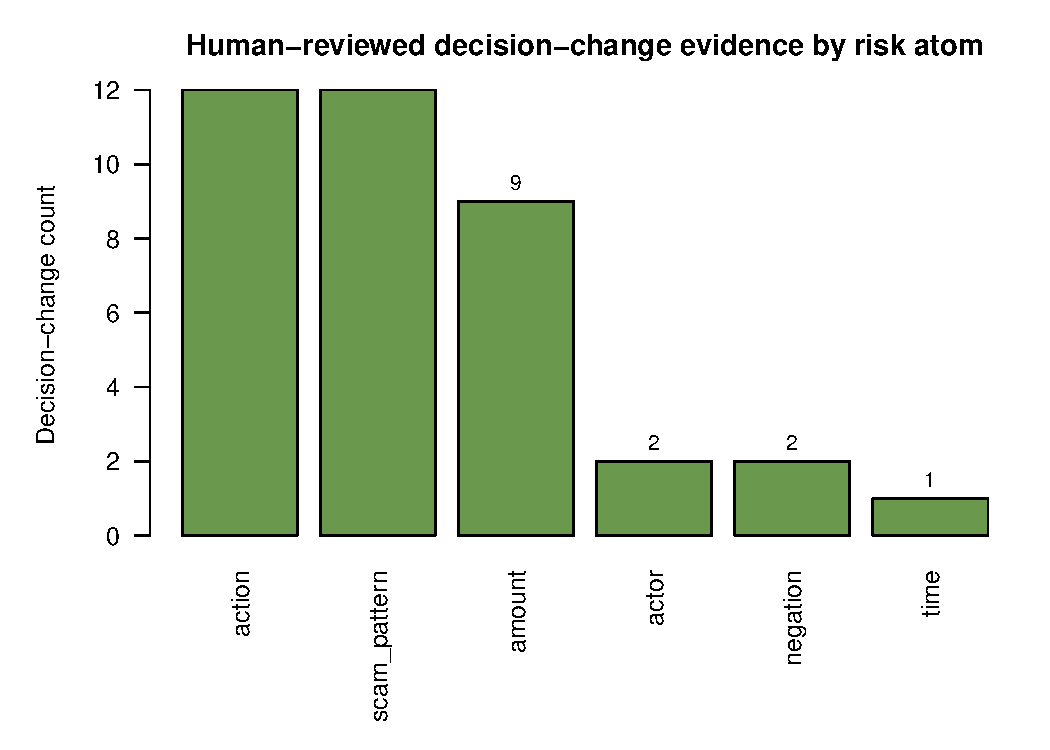
\includegraphics[width=.9\linewidth]{figures/fig6_risk_atom_review.pdf}
\caption{Human-reviewed decision-change evidence by risk atom. Source artifact: \artifact{70_experiments/runs/janus_300_high_stakes_human_audit_selection_2026_05_25/human_audit_risk_atom_review.tsv}.}
\label{fig:risk_atom}
\end{figure}
